\author{Andrei Tkachuk}
\part{Приложение функции нескольких переменных}
\section{Касательные к пространственным прямым и касательные к поверхностям}
		\begin{Def}[Касательная к пространственным кривым]
			Пусть $L$ --- гладкая пространственная кривая без особых точек или
			\begin{align*}
				&L : 
				\begin{cases}
					x = x(t) \\
					y = y(t) \\
					z = z(t) \\
				\end{cases} t \in U(t_0) \\ 
				&x(t), y(t), z(t) \in C'(U(t_0)) \\ 
				&(x'_t, y'_t, z'_t) \neq (0, 0, 0) 
			\end{align*}
		\end{Def}   
        Геометрически выглядит следующим образом
        \begin{figure}[bh]
            \noindent\centering{
                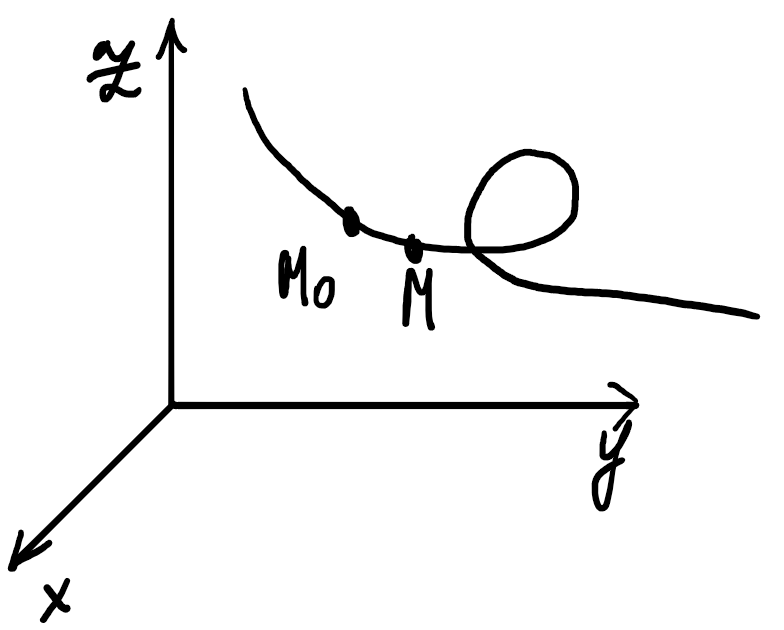
\includegraphics[width=75mm]{1_1_1.png}
                \caption{}
            }
        \end{figure}
		\begin{align*}
			&M_0(x_0, y_0, z_0) при t = t_0\\
			&\Delta t \neq 0, \; t = t_0 + \Delta t, \; \Delta t \in  U(t_0)\\
			&MM_0 : \frac{x - x_0}{x (t_0 + \Delta t) - x_0} = \frac{y - y_0}{y (t_0 + \Delta t) - y_0} = \frac{z - z_0}{z (t_0 + \Delta t) - z_0}
		\end{align*}
		Равенство выше является какноническим, если разделить элементы на $\Delta t$ и рассмотреть $\Delta t \rightarrow 0$ то получим следующее
		\begin{align*}
			&l_0 \: : \frac{x - x_0}{x'_0} = \frac{y - y_0}{y'_0} = \frac{z - z_0}{z'_0}\\
			&\text{так как : }\frac{x(t_0 - \Delta t) - x(t_0)}{\Delta t} \to x'_t(t_0) = x'_0 \; \text{при } \Delta t \to 0 \\
		\end{align*}
		$l_0$ --- касательная к кривой $L$ в точке $M_0$ \\
		$l_0$ --- прямая линия в пространстве ${x'_0}^2 + {y'_0}^2 + {z'_0}^2 \neq 0$
		
		
		\begin{Def}[Касательная плоскость к поверхности]
			Пусть $S : F(x, y, z) = 0$ --- поверхность в пространстве. $F(x, y, z)$ --- непрерывная функция в окрестности точки $M_0(x_0, y_0, z_0) \in S$\\
			Плоскость $\pi : Ax + By + Cz + D = 0$, где $A^2 + B^2 + C^2 \neq 0$ называется касательная плоскость к $S$ в точке $M_0$ если
			\begin{enumerate}
				\item $M_0 \in \pi$ 
				\item $\forall $ кривая линия $L \subset S, M_0 \in L$ гладкой кривой с касательным вектором $\vec{\tau} \neq \vec{0}$ выполняется условие $\vec{n} \perp \vec{\tau}, \vec{n} = {A, B, C}$ т.е. $(\vec{n}, \vec{\tau}) = 0$
			\end{enumerate}
			
         	\begin{figure}[bh]
            \noindent\centering{
                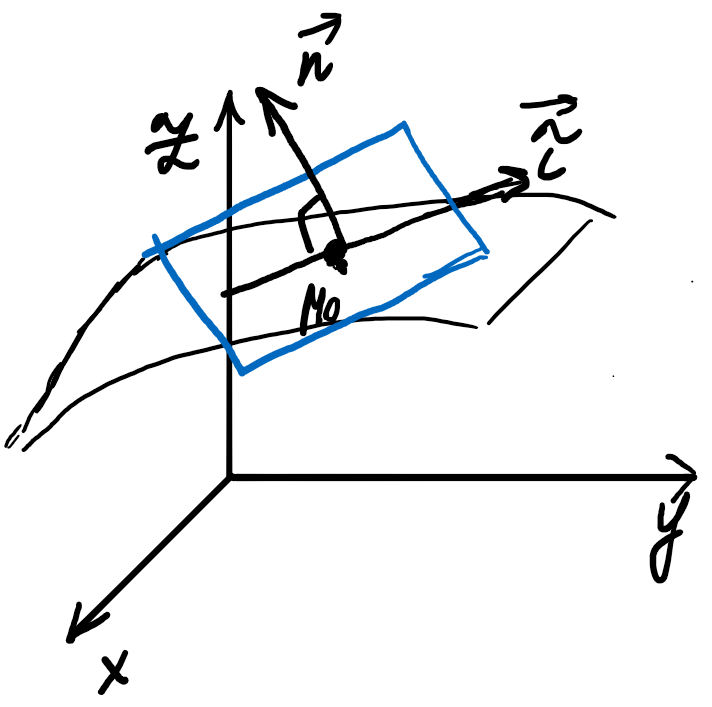
\includegraphics[width=65mm]{1_1_2.png}
                \caption{}
            }
            \end{figure}
						
		\end{Def}
	
		\begin{Th}[О существовании касательной плоскости]
			Пусть $F(x, y, z) \in C'(U(M_0))$, причём ${F'_x}^2(M_0) + {F'_y}^2(M_0) + {F'_z}^2(M_0) \neq 0$ \\
			Тогда для поверхности $S : F(x, y, z) = 0, \; M_0(x_0, y_0, z_0) \in S$ существует касательная плоскость $\pi : F'_x(M_0)\,(X-x_0) + F'_y(M_0)\,(Y-y_0) + F'_z(M_0)\,(Z-z_0) = 0$
		\end{Th}
		\begin{Proof}
			\begin{align*}
			&L:\begin{cases}
					x = x(t)\\
					y = y(t)\\
					z = z(t)\\	
			   \end{cases} \; t \in U(t_0) \quad x(t),\, y(t),\, z(t) \in C'(U(t_0))\\
			&x_0 = x(t_0), \; y_0 = y(t_0), \; z_0 = z(t_0), \quad M_0(x_0,\, y_0,\, z_0) \in L\\
			&\vec{\tau} = {x'_t(t_0),\, y'_t(t_0),\, z'_t(t_0)}\\
			&\vec{n} = {F'_x(M_0),\, F'_y(M_0),\, F'_z(M_0)}\\
			&\text{Докажем, что скалярное произведение равно нулю}\\
			&L \subset S \Rightarrow \forall t \in U(t_0) \; F(x(t),\, y(t),\, z(t)) = 0\\
			&\text{Из дифференцируемости сложной функции получаем}\\
			&(F(x(t),\, y(t),\, z(t)))'_t = F'_x\, x'_t + F'_y\, y'_t + F'_z\, z'_t\\ &\text{при} \; t = t_0\\
			&F'_x(M_0)\,x'_t(t_0) + F'_y(M_0)\,y'_t(t_0) + F'_z(M_0)\,z'_t(t_0) = 0 \; \Rightarrow \; (\vec{n}, \vec{\tau}) = 0\\
			&\Rightarrow \; \pi : F'_x(M_0)\,(X-x_0) + F'_y(M_0)\,(Y-y_0) + F'_z(M_0)\,(Z-z_0) = 0
			\end{align*}
		\end{Proof}
		
		\begin{Def}[Градиент]
			$\{F'_x(M_0);\; F'_y(M_0);\; F'_z(M_0)\} = \grad{F}{M_0}$ --- градиент функции $F$ в точке $M_0$
		\end{Def}
	
		\begin{Th}[Существование касательной плоскости]
            Рассматривается случай явно заданной поверхности\\
			Пусть $f(x, y) \in C'(U(N_0)), \, N_0(x_0,\, y_0)$.\\
			Тогда для явно заданной поверхности $S : z = f(x, y)$ существует касательная плоскость в точке $M_0(x_0,\, y_0,\, z_0), \, \text{где} z_0 = f(N_0)$ вида 
			\[\pi: Z-z_0 = f'_x(N_0)\,(X-x_0) + f'_y(N_0)\,(Y-y_0)\]
		\end{Th}
		\begin{Proof}
			\begin{align*}
				&S: f(x, y) - z = 0, \, F = f(x, y) - z\\
				&F'_x = (f(x, y) - z)'_x = f'_x(N) \\ 
				&\text{Аналогично для других производных}\\
				&F'_y = f'_x(N); \; F'_z = -1;\\
				&\text{Т.к. мы задали явную функцию $F$, то по теореме 1 получаем}\\
				&\pi : f'_x(N_0)(X-x_0) + f'_y(N_0)(Y-y_0) + f'_z(N_0)(Z-z_0) = 0 \\
				&\pi : f'_x(N_0)(X-x_0) + f'_y(N_0)(Y-y_0) - (Z-z_0) = 0 ,\, \text{примечание } z_0 = f(x_0, y_0)\\
				&\pi : Z = f'(x_0, y_0) + f'_x(N_0)(X-x_0) + f'_y(N_0)(Y-y_0)
			\end{align*}
		\end{Proof}
		
		\begin{Def}[Нормаль к поверхности]
			Пусть $S : F(x,y,z) = 0, \; (x, y, z) \in U(M_0)$ гладкая поврхность. $M_0(x_0, y_0, z_0) \in S$.\\
			Тогда нормаль $n$ к поверхности $S$ в точке $M_0$ называется прямая линия $n,\, M_0 \in n,\, n\perp\pi$, где $\pi$ --- касательная плоскость
		\end{Def}
		
		\begin{Note}
			Если в условии определения 4 $ \grad{F}{M_0} \neq \Vectr{0}$, то каноническое уравнение $n$
			\[
				n : \frac{x - x_0}{F'_x(M_0)} = \frac{y - y_0}{F'_y(M_0)} = \frac{z - z_0}{F'_z(M_0)}
			\] 
		\end{Note}
		